\chapter{Слежение и компенсация по выходу}
\label{ch:chap3}
\section{Условие задачи}


Рассмотрим систему, состоящую из объекта управления, генератора внешнего воздействия и виртуального выхода:
$$
  \begin{cases}
    \dot{x} = Ax + Bu + B_f w, \tab x(0)= \begin{bmatrix} 0 & 0 & 0 \end{bmatrix}^T, \\
    y = Cx + Dw, \\
    \dot{w} = \text{Г}w, \tab w(0) = \begin{bmatrix} 1 & 1 & 1 & 1 \end{bmatrix}^T 
  \end{cases}
$$ и выполним следующие шаги:

\begin{itemize}
  \item Найти собственные числа матрицы \text{Γ} и определить характер внешнего возмущения.
  \item Проверим матрицы $\vec{CD}, \vec{AB}$  на обнаруживаемость и сделать вывод о возможности
  осуществления слежения и компенсации по выходу.
  \item Построить схему моделирования системы, замкнутой регулятором, состоящим
  из расширенного наблюдателя и закона управления $u = K_1 \hat{x_1} + K_2 \hat{w}$,  обеспечивающего выполнение целевого условия при внешнем воздействии, 
  задаваемом генератором.
  \item Синтезировать «feedback»-компоненту $K_1$ следящего регулятора. Привести выкладки процедуры синтеза и
  полученную матрицу $K_1$.
  \item Синтезировать матрицу коррекции $L$ наблюдателя. Привести выкладки процедуры
  синтеза и полученную матрицу $L$. 
  \item Рассмотреть два случая виртуального выхода:
  \begin{itemize}
    \item $z = C_Z x + D_z w$
    \item $z = y $.
  \end{itemize}
  \item   Для каждого из вариантов виртуального выхода:
  \begin{itemize}
    \item Синтезировать «feedforward»-компоненту $K_2$ следящего регулятора. Привести выкладки процедуры синтеза и полученную матрицу $K_2$.
    \item Выполнить моделирование, состоящее из трёх частей.
    \item Найти собственные числа матрицы наблюдателя $\vec{A}$ и сравнить с 
    собственными числами матрицы генератора \text{Γ}.
    
  \end{itemize}
  \item  Проанализировать полученные результаты и сделать выводы.
\end{itemize}

\section{Решение задания}

Представим уравнения текущего регулятора в форме $\text{В-С-В}$, где $y(t)$ - вход, а $u(t)$ - выход:

$$
  \begin{cases}
    \dot{\hat{x}} = A \hat{x} + Bu + B_f \hat{w} + L_x (\hat{y} - y) \\
    \dot{\hat{w}} = \text{Г} \hat{w} + L_w (\hat{y} - y) \\
    \hat{y} = C\hat{x} + D \hat{w} \\
    u = K_1 \hat{x} + K_2 \hat{w}
  \end{cases}
$$
$$
  \begin{cases}
    \begin{bmatrix}
      \dot{\hat{x}} \\ \dot{\hat{w}} 
    \end{bmatrix} = 
                    \begin{bmatrix}
                      A + B K_1 +L_x C & B K_2 + B_f + L_x D \\
                      L_w C            &  \text{Г} + L_w D
                    \end{bmatrix} - \begin{bmatrix}
                      L_x \\ L_w
                    \end{bmatrix} y \\
    u = K_1 \hat{x} + K_2 \hat{w}
  \end{cases}
$$


В итоге:
$$
  \bar{A^*} = \begin{bmatrix}
                A + B K_1 +L_x C & B K_2 + B_f + L_x D \\
                L_w C            &  \text{Г} + L_w D
              \end{bmatrix}
$$

$$
  \sigma(\text{Г}) = \{ \pm 3i, \pm 2i \}
$$
Характер внешнего возмущения остался с прошлых заданий: частоты $\omega = 2$ и $\omega = 3$.

Проверим матрицы $\vec{CD} =\begin{bmatrix} C & D \end{bmatrix}$ и $\vec{AB} = \begin{bmatrix} A & B_f \\ 0 & \text{Г} \end{bmatrix}$ 
на обнаруживаемость, воспользуемся для этого критерием Хаутуса:

$$
    rank \begin{pmatrix}
        \vec{AB} - 3\pm 3j \\ \vec{CD}
    \end{pmatrix} = 7 
$$
$$
    rank \begin{pmatrix}
        \vec{AB} - 2 \\ \vec{CD}
    \end{pmatrix} = 7 
$$
$$
    rank \begin{pmatrix}
        \vec{AB} \pm 3j \\ \vec{CD}
    \end{pmatrix} = 7 
$$
$$
    rank \begin{pmatrix}
        \vec{AB} \pm 2j \\ \vec{CD}
    \end{pmatrix} = 7 
$$
В итоге критерий выполняется,  расширенная система полностью наблюдаема, значитм можно 
осуществить слежение и компенсацию по выходу.



Построим схему моделирования системы,  замкнутой регулятором, состоящим из расширенного наблюдателя:
$$
    \begin{bmatrix}
      \dot{\hat{x}} \\ \dot{\hat{w}}
    \end{bmatrix} = \bar{A} 
                      \begin{bmatrix}
                        \hat{x} \\ \hat{w}
                      \end{bmatrix}
                      - Ly
$$
и закона управления:
$$
   u = K_1 \hat{x} + K_2 \hat{w}
$$
обеспечивающего выполнение целевого условия  при внешнем воздействии, задаваемом генератором.

\begin{figure}[ht]
  \centering
  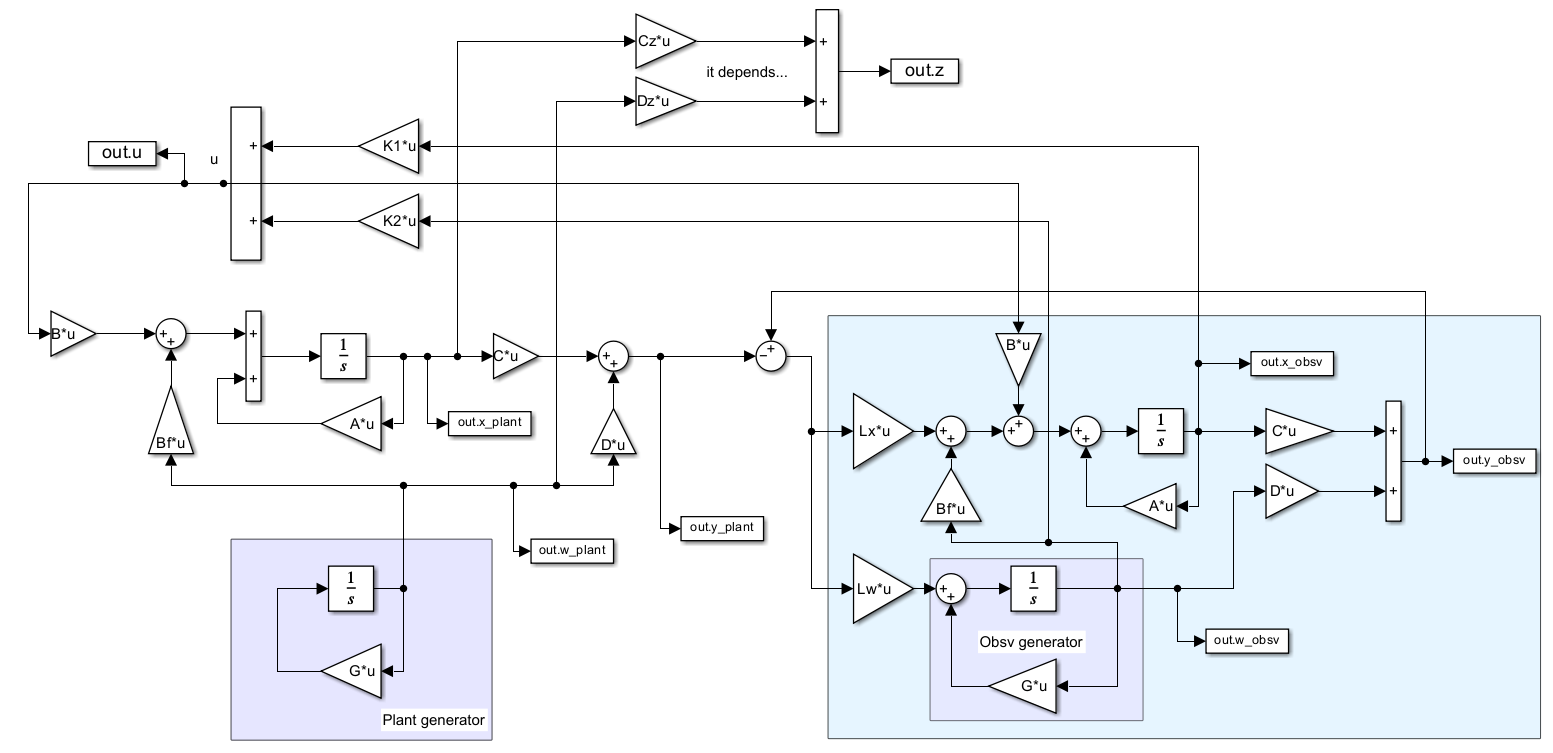
\includegraphics[width=1.0\textwidth]{scheme3.png}
  \caption{Схема - слежение и компенсация по выходу}
\end{figure}


Синтезируем «feedback»-компоненту $K_1$ с помощью \text{LQR}-регулятора, функционал качества:
$$
  J = \int_0^{\infty} (x^TQx + u^TRu) dt
$$ 
Параметры останутся теми же:
$$
  Q = \begin{bmatrix}
    1 & 0 & 0 \\
    0 & 1 & 0 \\
    0 & 0 & 1
  \end{bmatrix}, \quad R = \begin{bmatrix}
    1
  \end{bmatrix}
$$
Получаем матрицу $K_1$:
$$
  K_1 = \begin{bmatrix}
    8.71 & -8.62 & 8.47 \\
\end{bmatrix}
$$

Таким же подходом синтезируем матрицу коррекции наблюдателя $L$ параметры также возьмём все единичные правда лишь размерности немного увеличатся:
$$
  R = 1, \tab Q = I_{7 \times 7}
$$
$$ 
L = \begin{bmatrix}
  -133.27 \\
  -105.92 \\
  81.86 \\
  18.48 \\
  27.96 \\
  12.11 \\
  -21.25 \\
\end{bmatrix}
$$

\newpage
\subsection{Первый виртуальный выход}
$$
  z = C_Z x + D_Z w
$$




Синтезируем «feedforward»-компоненту $K_2$:
$$
  K_2 = \begin{bmatrix}
    14.09 & -7.14 & 7.5 & 9.16 \\
\end{bmatrix}
$$


\begin{figure}[ht]
  \centering
  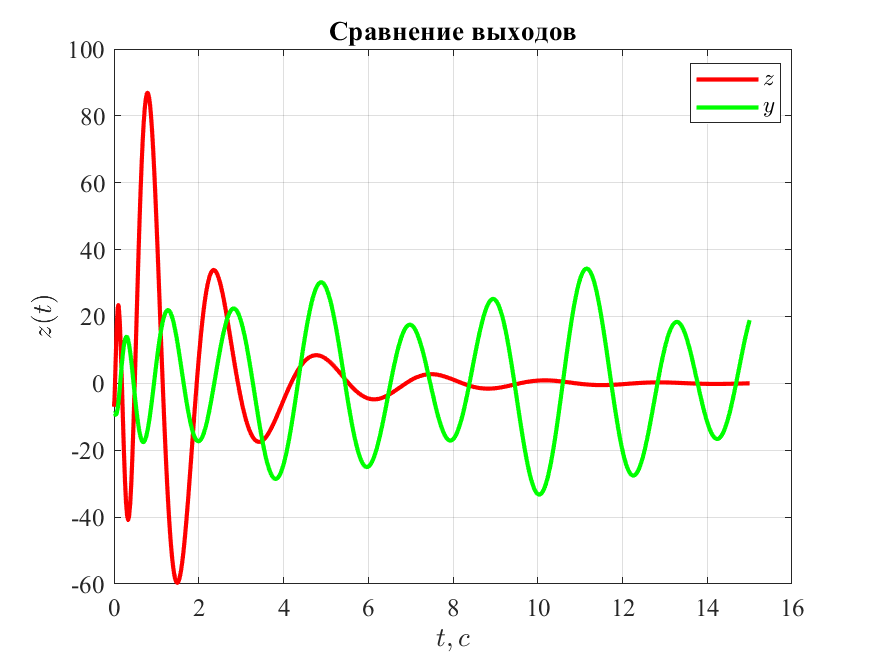
\includegraphics[width=0.8\textwidth]{yz1.png}
  \caption{Моделирование - вектор фактического и виртуального выхода, $z = C_Z x + D_Z w$}
\end{figure}
\newpage
\begin{figure}[ht]
  \centering
  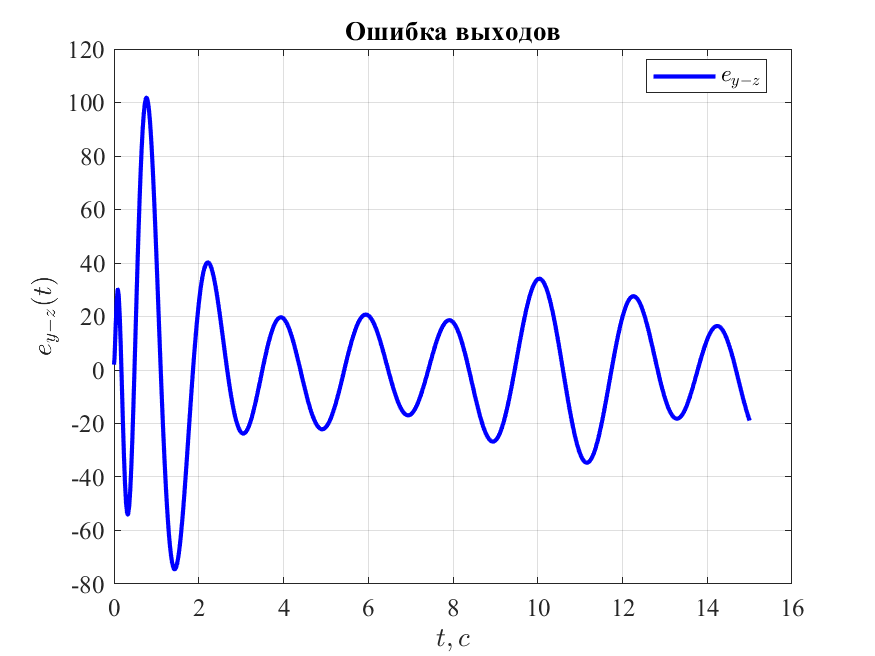
\includegraphics[width=0.8\textwidth]{e_yz1.png}
  \caption{Моделирование - ошибка между фактическим-виртуальным выходом, $z = C_Z x + D_Z w$}
\end{figure}


\begin{figure}[ht]
  \centering
  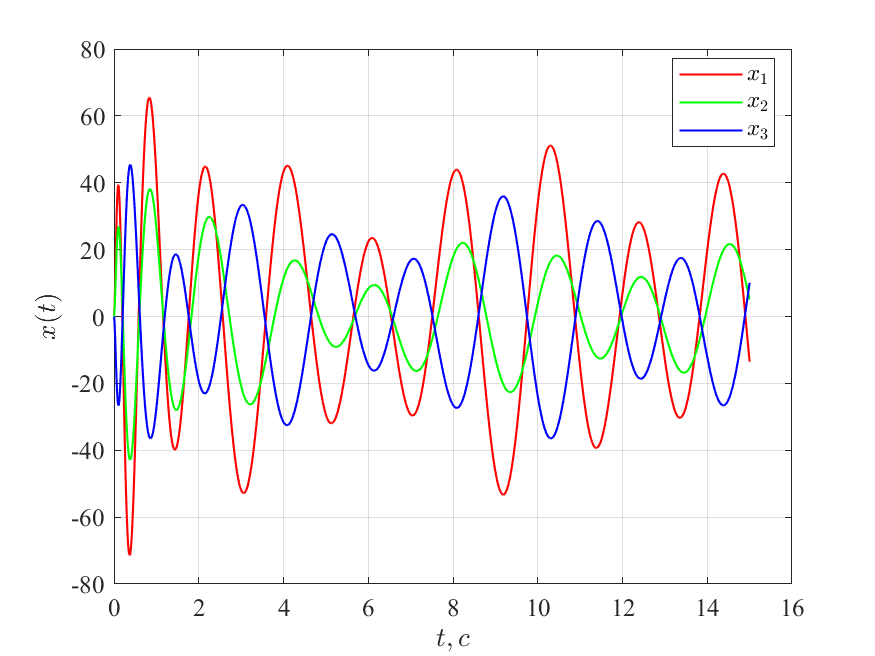
\includegraphics[width=0.8\textwidth]{plant_x1.png}
  \caption{Моделирование - $x(t)$, $z = C_Z x + D_Z w$}
\end{figure}

\begin{figure}[ht]
  \centering
  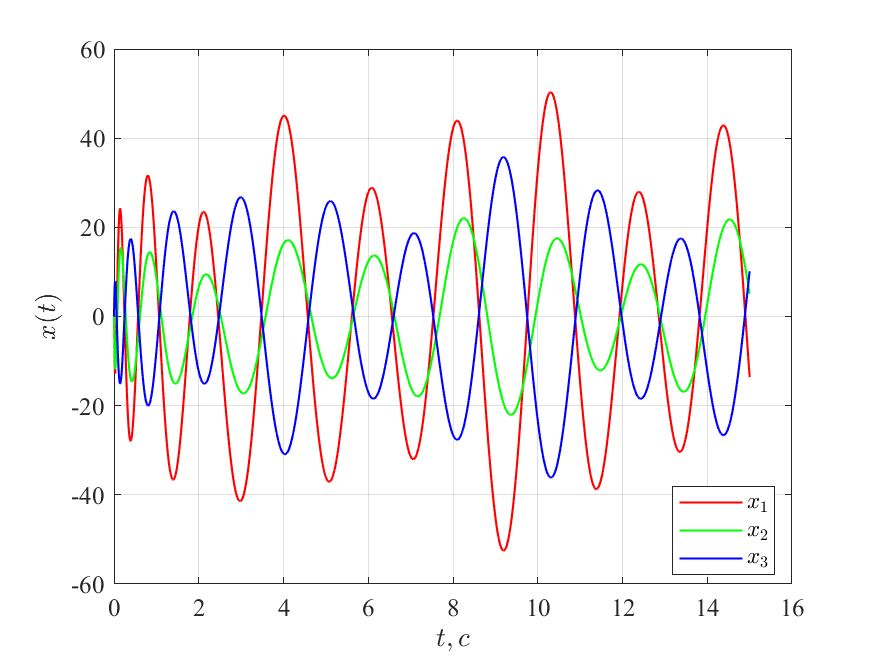
\includegraphics[width=0.8\textwidth]{obsv_x1.png}
  \caption{Моделирование - $\hat{x}(t)$, $z = C_Z x + D_Z w$}
\end{figure}


\begin{figure}[ht]
  \centering
  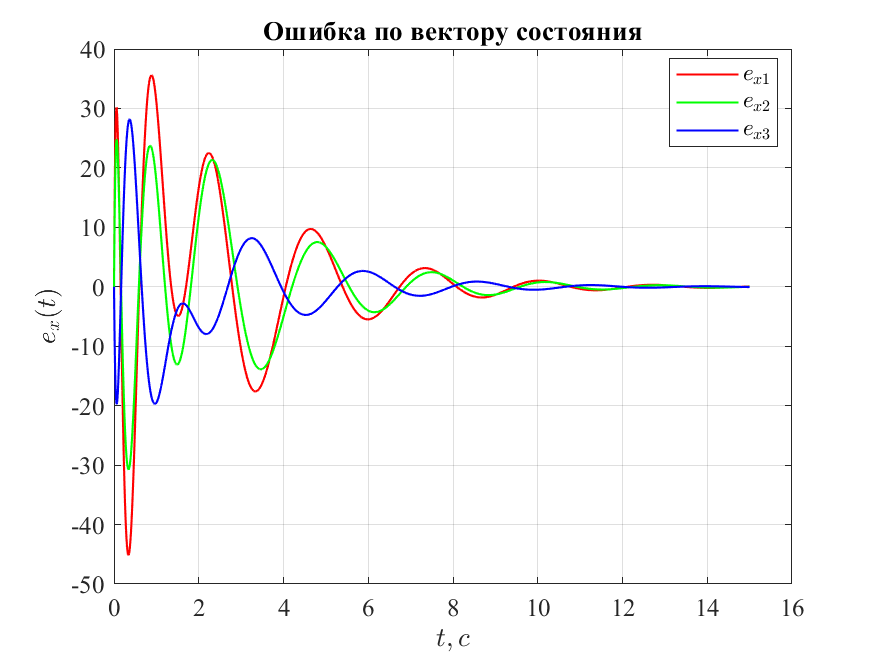
\includegraphics[width=0.8\textwidth]{e_x1.png}
  \caption{Моделирование - ошибка наблюдателя вектора состояния, $z = C_Z x + D_Z w$}
\end{figure}
\newpage
\begin{figure}[ht]
  \centering
  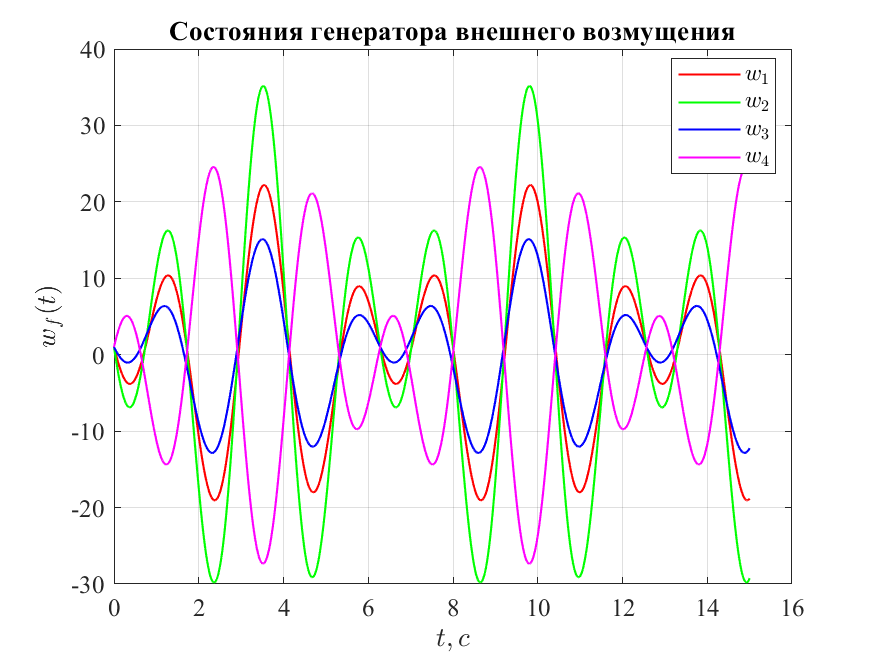
\includegraphics[width=0.8\textwidth]{plant_w1.png}
  \caption{Моделирование - $w(t)$, $z = C_Z x + D_Z w$}
\end{figure}


\begin{figure}[ht]
  \centering
  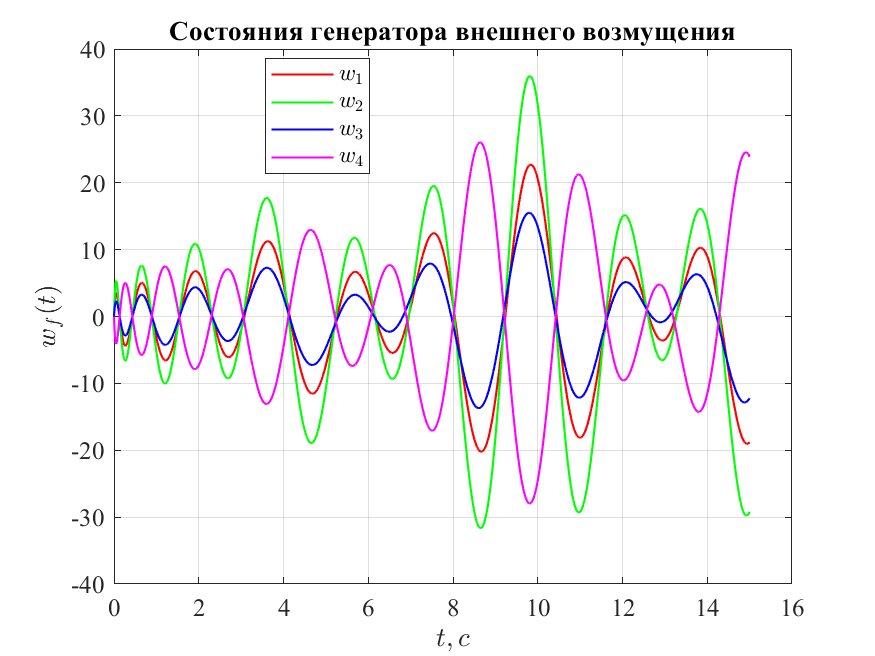
\includegraphics[width=0.8\textwidth]{obsv_w1.png}
  \caption{Моделирование - $\hat{w}(t)$, $z = C_Z x + D_Z w$}
\end{figure}

\newpage
\begin{figure}[ht]
  \centering
  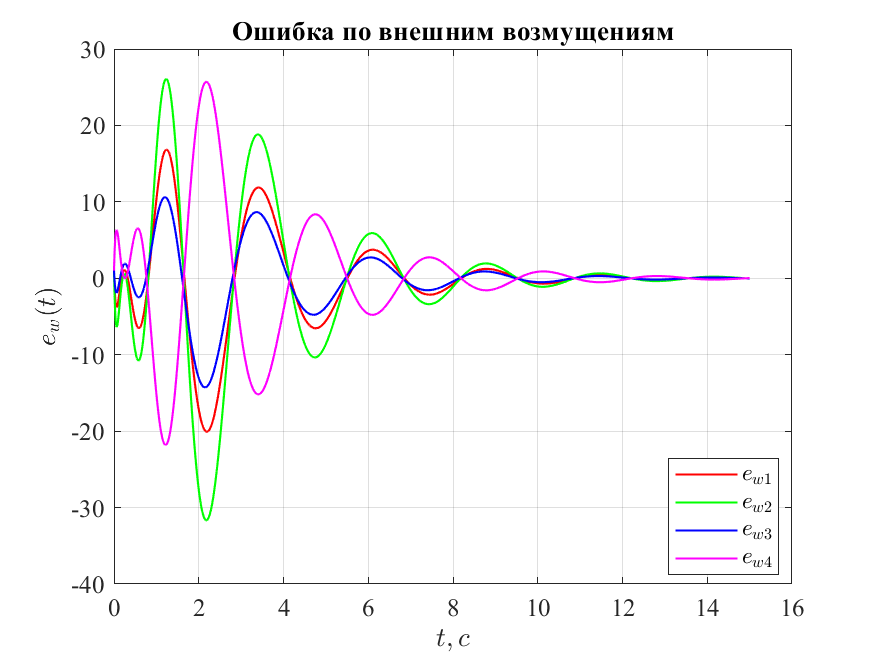
\includegraphics[width=0.8\textwidth]{e_w1.png}
  \caption{Моделирование - ошибка наблюдателя внешнего возмущения, $z = C_Z x + D_Z w$}
\end{figure}

\newpage
\begin{figure}[ht]
  \centering
  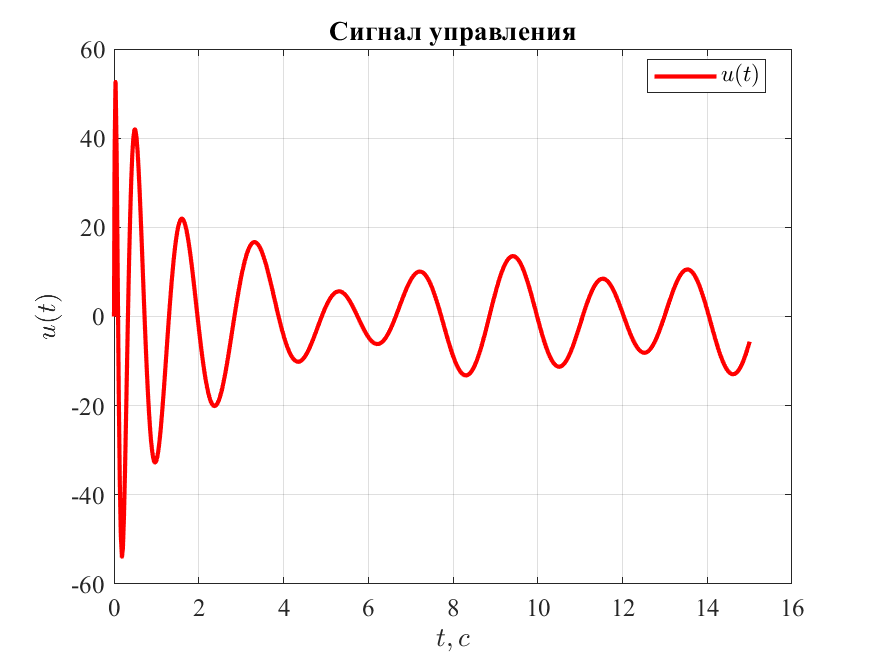
\includegraphics[width=0.8\textwidth]{u7.png}
  \caption{Моделирование - управляющий сигнал, $z = C_Z x + D_Z w$}
\end{figure}

Найдём собственные числа матрицы системы регулятора в форме \text{В-С-В}:
$$
  \sigma(\bar{A^*}) = \{ -21 \pm 26.41j, -0.1 \pm 24.6j, -0.46 \pm 1.41j , -2.07 \}
$$

Как можно заметить, никаких совпадений со  спектром матрицы генератора $G$ нет. 


\clearpage
\newpage
\subsection{Второй виртуальный выход}
$$
  z = y = Cx + Dw
$$

Синтезируем «feedforward»-компоненту $K_2$:
$$
  K_2 = \begin{bmatrix}
    -16 & 17.39 & -4.53 & 6.62 \\
\end{bmatrix}
$$

\begin{figure}[ht]
  \centering
  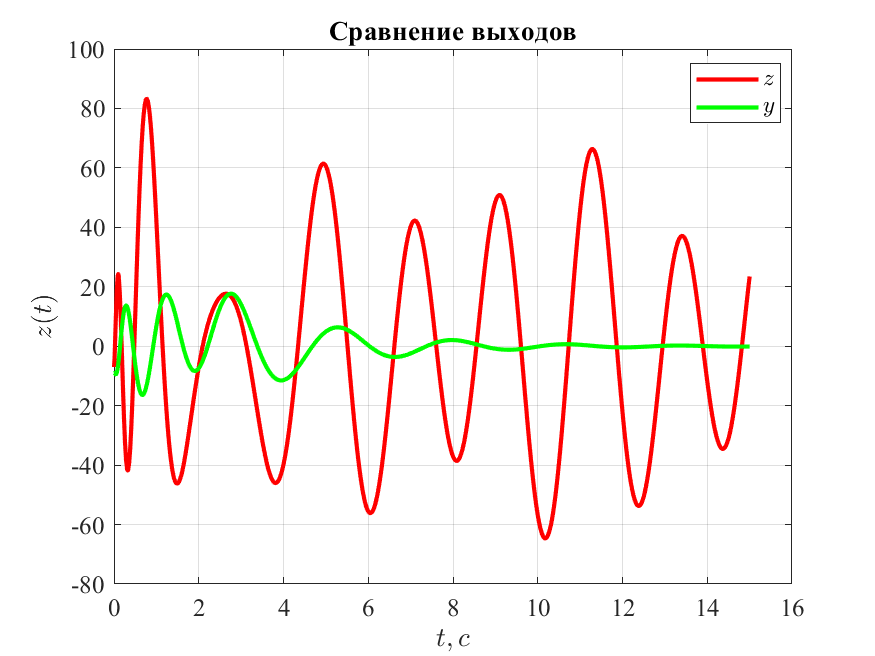
\includegraphics[width=0.8\textwidth]{yz2.png}
  \caption{Моделирование - вектор фактического и виртуального выхода, $z = y$}
\end{figure}
\newpage
\begin{figure}[ht]
  \centering
  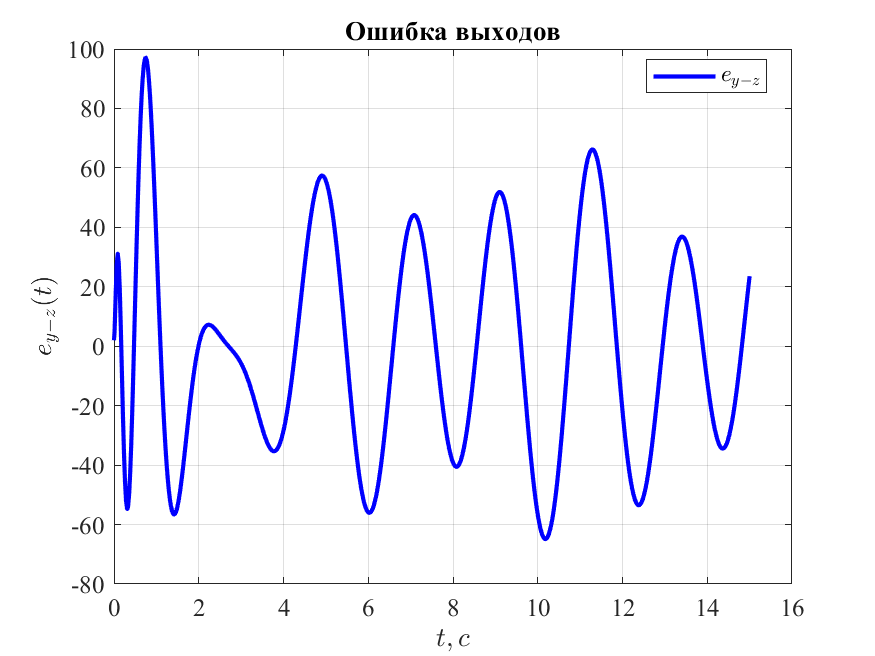
\includegraphics[width=0.8\textwidth]{e_yz2.png}
  \caption{Моделирование - ошибка между фактическим-виртуальным выходом, $z = y$}
\end{figure}


\begin{figure}[ht]
  \centering
  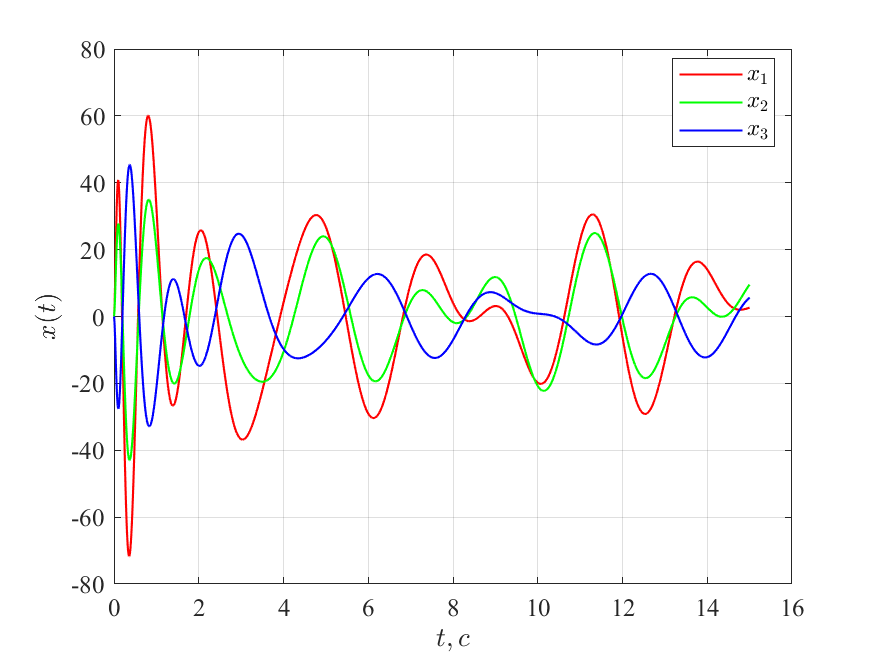
\includegraphics[width=0.8\textwidth]{plant_x2.png}
  \caption{Моделирование - $x(t)$, $z = y$}
\end{figure}
\newpage
\begin{figure}[ht]
  \centering
  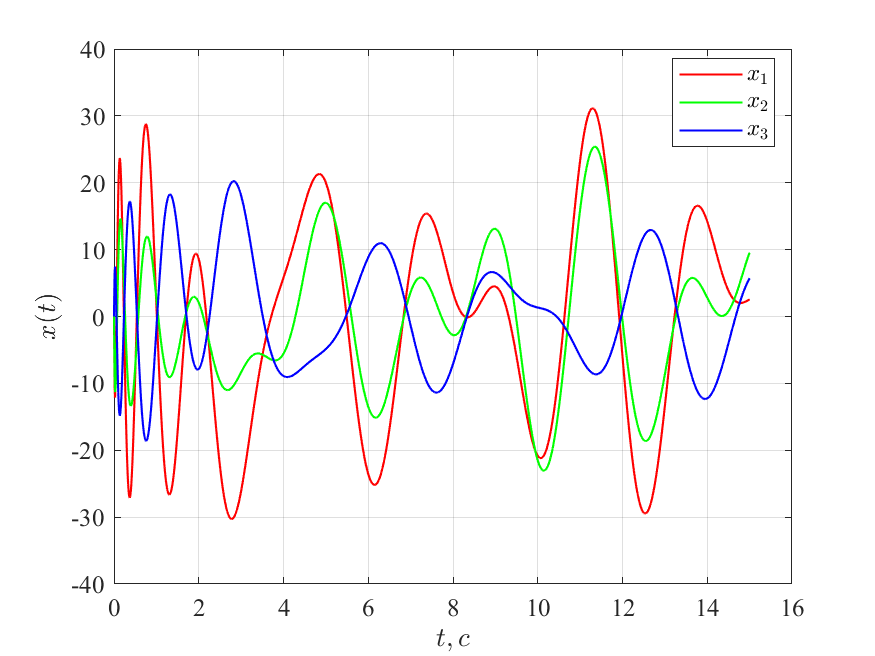
\includegraphics[width=0.8\textwidth]{obsv_x2.png}
  \caption{Моделирование - $\hat{x}(t)$, $z = y$}
\end{figure}


\begin{figure}[ht]
  \centering
  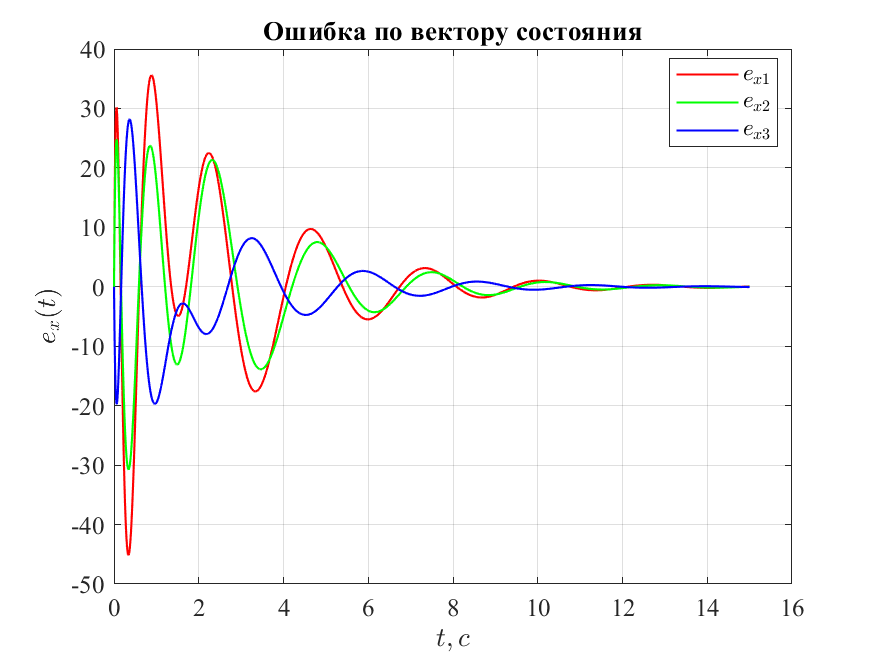
\includegraphics[width=0.8\textwidth]{e_x2.png}
  \caption{Моделирование - ошибка наблюдателя вектора состояния, $z = y$}
\end{figure}
\newpage
\begin{figure}[ht]
  \centering
  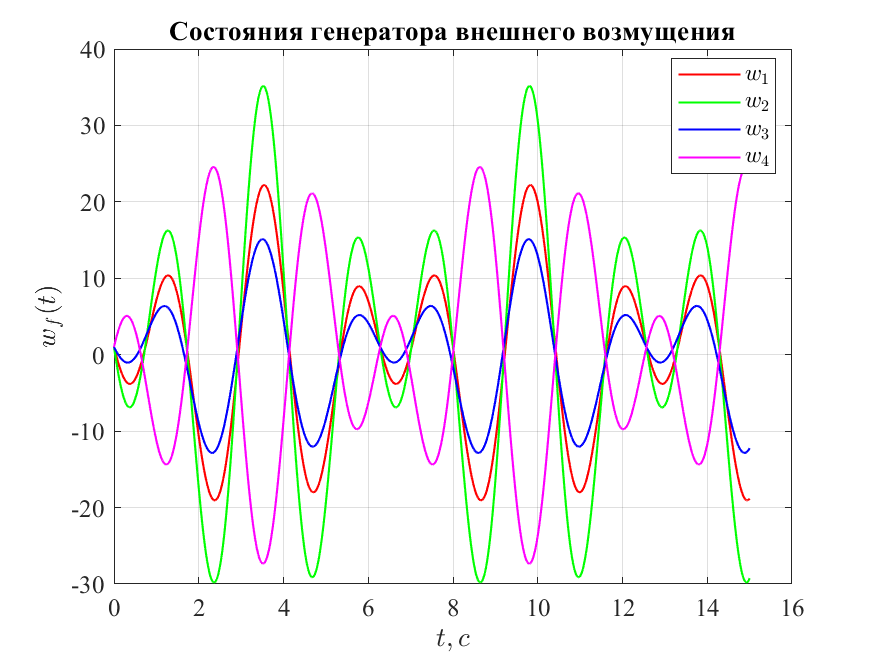
\includegraphics[width=0.8\textwidth]{plant_w2.png}
  \caption{Моделирование - $w(t)$, $z = y$}
\end{figure}


\begin{figure}[ht]
  \centering
  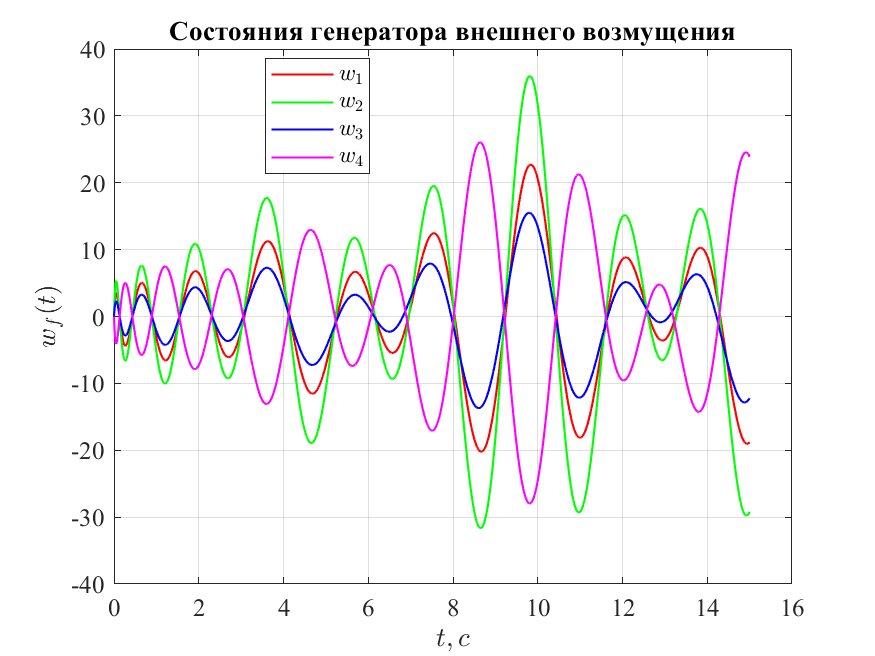
\includegraphics[width=0.8\textwidth]{obsv_w2.png}
  \caption{Моделирование - $\hat{w}(t)$, $z = y$}
\end{figure}

\newpage
\begin{figure}[ht]
  \centering
  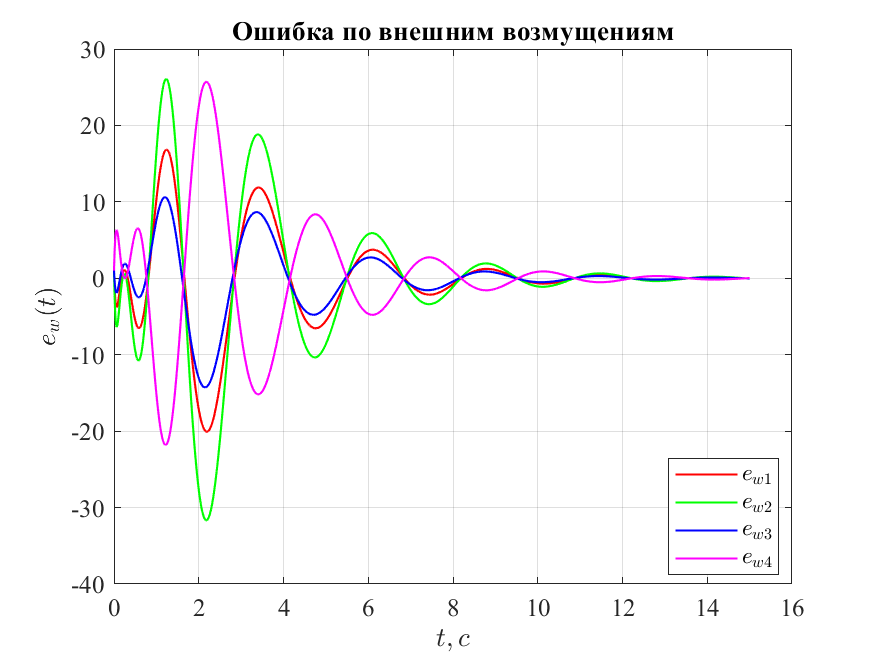
\includegraphics[width=0.8\textwidth]{e_w2.png}
  \caption{Моделирование - ошибка наблюдателя внешнего возмущения, $z = y$}
\end{figure}


\begin{figure}[ht]
  \centering
  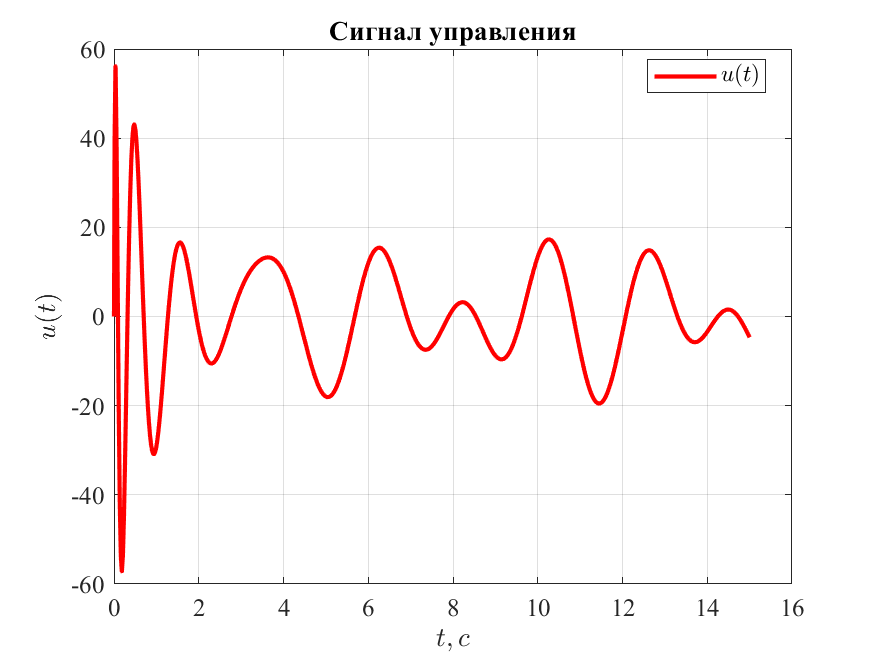
\includegraphics[width=0.8\textwidth]{u8.png}
  \caption{Моделирование - управляющий сигнал, $z = y$}
\end{figure}

Найдём собственные числа матрицы системы регулятора в форме \text{В-С-В}:
$$
  \sigma(\bar{A^*}) = \{ -22 \pm 27.5j, \pm 3j, \pm 2j, -2.02 \}
$$

Как можно заметить, спектр матрицы системы регулятора содержит в себе спектр матрицы генератора $G$. 
Принцип внутренней модели выполняется.



\section{Выводы}

В этом задании мы мы рассмотрели расширенный наблюдатель системы, 
который давал оценки не только состояния системы, но и генератора возмущений, 
решали мы задачу слежения и компенсации относительно этих  оценок.
\endinput